\documentclass[12pt]{article}
\usepackage{graphicx}
\title{Experiment 1: XOR and Full Adder}
\author{Annirudh K P, Roll Number 210070009}
\date{August 7, 2022}
\begin{document}

\maketitle

\section{Overview of the experiment/assignment}

In this experiment, we were introduced to VHDL, a hardware description language used to program stimulations of different digital components. The problem statement of this experiment is to design the XOR and the Full Adder, and then describe them in VHDL using structural modelling. We were given only NAND gates to use, and no, nobody felt it was cute. The objective of this experiment was to understand the Quartus Design Flow, and give us hands on experience over different technical glitches/problems we may face in this piece of software which has been made unwantedly hard.

\section{Experimental setup}

\subsection{Design Requirements}
\subsubsection{XOR Gate}
XOR gate (Exclusive OR gate) takes 2 inputs and gives true only when one of the input is low and other is high, and rest is false. Truth table is given below.

\begin{table}
 \centering
\begin{tabular}{|c  c |c|} 
\hline  
A & B & Output \\
\hline
0 & 0 & 0 \\
0 & 1 & 1 \\
1 & 0 & 1 \\
1 & 1 & 0 \\
\hline
\end{tabular}
\caption{Truth Table for XOR gate}
\end{table}

\subsubsection{Full Adder}
\paragraph{}
Full Adder takes in 3 inputs, namely A, B and a carry C. And it gives out 2 output, one Carry and other is Sum.

\paragraph{}
Full Adder is generally made by two Half Adders, when we connect them in series with Sum of First Half Adder and the Carry C to two inputs of 2nd Half Adder. We then get Sum and Carry.

\paragraph{}
Truth Table of Full Adder is given below in the Table.

\begin{table}
 \centering
\begin{tabular}{|c  c  c | c | c|} 
\hline  
A & B & C & Sum & Carry \\  
\hline  
0 & 0 & 0 & 0 & 0 \\  
0 & 0 & 1 & 1 & 0   \\  
0 & 1 & 0 & 1 & 0 \\ 
0 & 1 & 1 & 0 & 1 \\ 
1 & 0 & 0 & 1 & 0 \\  
1 & 0 & 1 & 0 & 1 \\
1 & 1 & 0 & 0 & 1 \\ 
1 & 1 & 1 & 1 & 1 \\ 
\hline
\end{tabular}
\caption{Truth Table for Full Adder}
\end{table}

\subsection{Design Schematics}
\begin{figure}[h]
  % will center the figure.
  % include graphics (can include eps, jpg, pdf ...)
  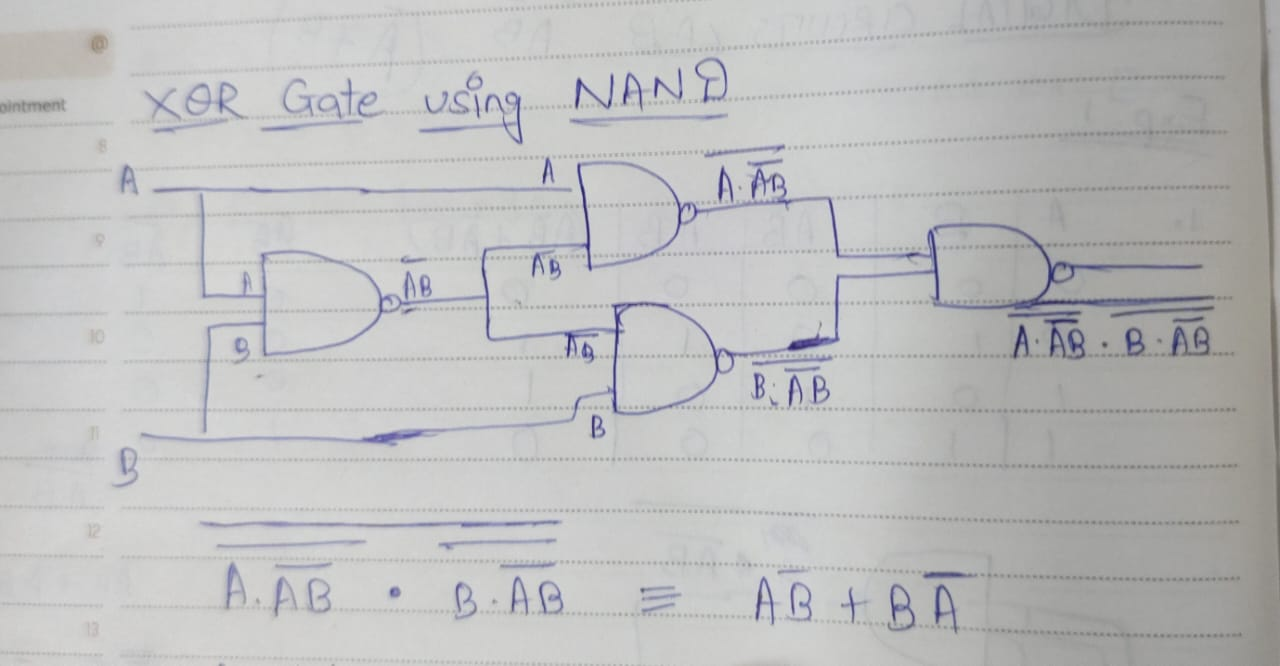
\includegraphics[scale=0.3]{images/XOR_DESIGN.jpeg}  % change scale factor to re-size the image.
  % give a caption.
  \caption{XOR gate using only NAND gates}
  % a label to refer to the figure
  \label{XOR_schematic}
\end{figure}
\begin{figure}[h]
  % include graphics (can include eps, jpg, pdf ...)
  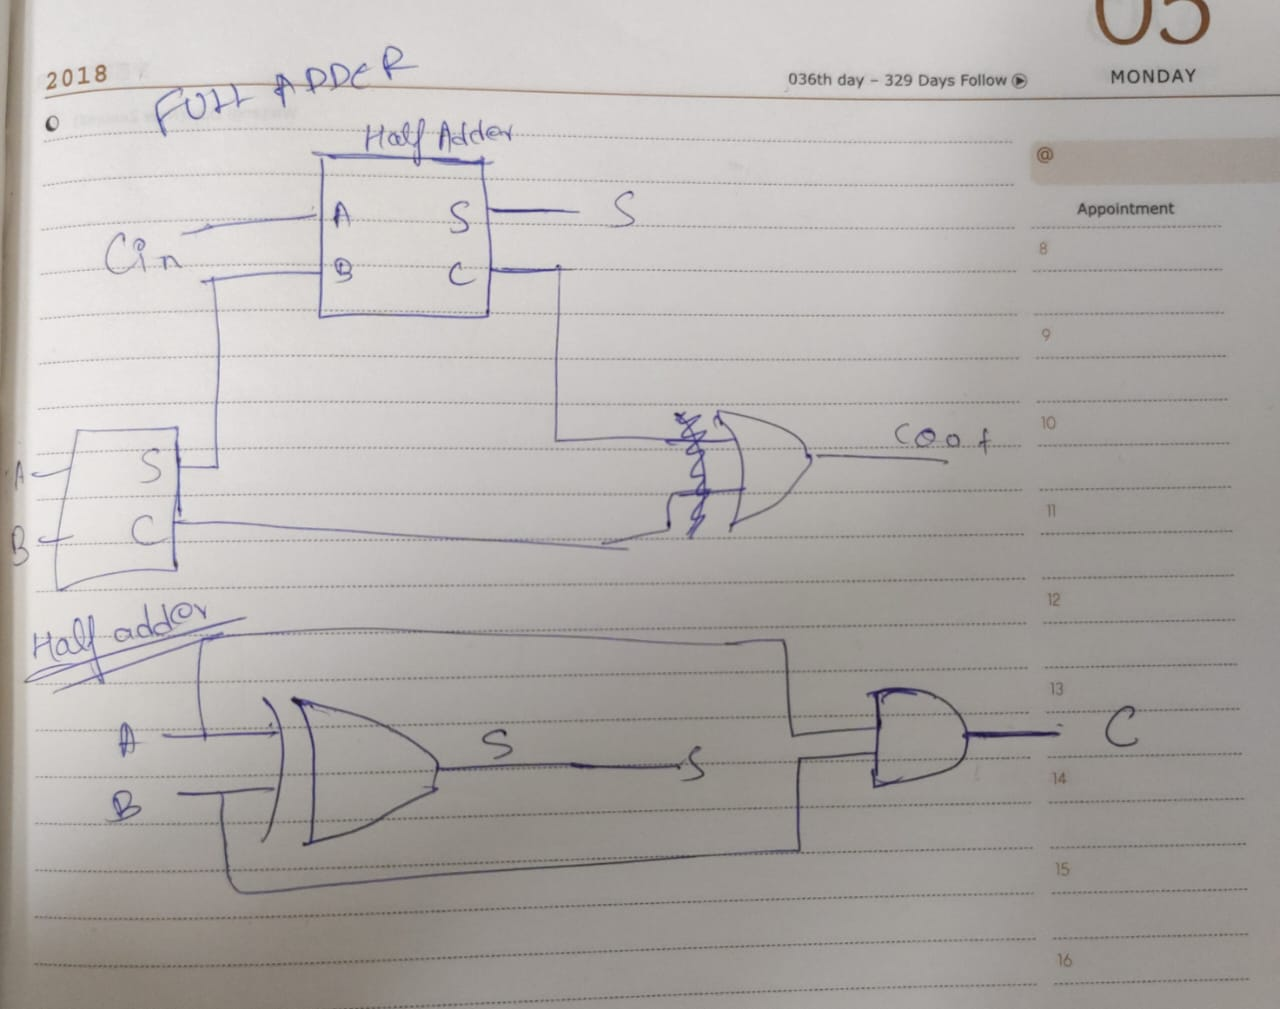
\includegraphics[scale=0.3]{images/FULLADDER_DESIGN.jpeg}  % change scale factor to re-size the image.
  % give a caption.
  \caption{Full Adder using only NAND and XOR gates}
  % a label to refer to the figure
  \label{Full_adder_schematic}
\end{figure}


\paragraph{}
Using only 5 NAND gates we can make a XOR gate. This gate we can also use while making a Full Adder.
\paragraph{}
In Full Adder Schematic I have used Half Adder and also the OR gate. Have defined entity-architecture pairs for the same and then used them.


\subsection{Code for XOR gate}

\begin{verbatim}
library ieee;
use ieee.std_logic_1164.all;
library work;
use work.Gates.all;

entity XOR_GATE  is
  port (A, B: in std_logic; OUTPUT: out std_logic);
end entity XOR_GATE;

architecture Struct of XOR_GATE is
  signal S1, S2, S3 : std_logic;
begin
  -- component instances
  NAND1: NAND_2 port map (A => A, B => B, Y => S1);
  NAND2: NAND_2 port map (A => A, B => S1, Y => S2);
  NAND3: NAND_2 port map (A => B, B => S1, Y => S3);
  
  -- final XOR
  NAND4: NAND_2 port map (A => S2, B => S3, Y => OUTPUT);
  
end Struct;
\end{verbatim}

\subsection{Code for Full Adder gate}
\begin{verbatim}

library ieee;
use ieee.std_logic_1164.all;
library work;
use work.Gates.all;

entity OR_GATE  is
  port (A, B: in std_logic; OUTPUT: out std_logic);
end entity OR_GATE;

architecture Struct of OR_GATE is
	signal A_BAR, B_BAR : std_logic;
begin
  -- component instances
  NAND1: NAND_2 port map (A => A, B => A, Y => A_BAR);
  NAND2: NAND_2 port map (A => B, B => B, Y => B_BAR);
  
  -- final OR
  NAND3: NAND_2 port map (A => A_BAR, B => B_BAR, Y => OUTPUT);
end Struct;

library ieee;
use ieee.std_logic_1164.all;
library work;
use work.Gates.all;


entity HALF_ADDER1 is
	port (A, B: in std_logic; SUM, C0: out std_logic);
end entity HALF_ADDER1;

architecture Struct1 of HALF_ADDER1 is
	signal S1, S2, S3, S0 : std_logic;
begin
	--carry
	NAND1: NAND_2 port map (A => A, B => B, Y => S0);
	NAND2: NAND_2 port map (A => S0, B => S0, Y => C0);
	
	--sum
	NAND3: NAND_2 port map (A => A, B => B, Y => S1);
	NAND4: NAND_2 port map (A => A, B => S1, Y => S2);
	NAND5: NAND_2 port map (A => B, B => S1, Y => S3);
	NAND6: NAND_2 port map (A => S2, B => S3, Y => SUM);

end Struct1;

library ieee;
use ieee.std_logic_1164.all;
library work;
use work.Gates.all;

entity FULL_ADDER is
	port (A, B, CI: in std_logic; SUM, CO: out std_logic);
end entity FULL_ADDER;

architecture Struct2 of FULL_ADDER is
	signal S1, C1, C2 : std_logic;
	component HALF_ADDER1 is
		port (A, B: in std_logic; SUM, C0: out std_logic);
	end component HALF_ADDER1;
	component OR_GATE is
		port (A, B: in std_logic; OUTPUT: out std_logic);
	end component;
begin
	HA_1: HALF_ADDER1 port map (A => A, B => B, SUM => S1, C0 => C1);
	HA_2: HALF_ADDER1 port map (A => CI, B => S1, SUM => SUM, C0 => C2);
	OR_1: OR_GATE port map (A => C1, B => C2, OUTPUT => CO);
end Struct2;

\end{verbatim}

\section{Observations}
 
We get waveform for corresponding to input and output which is given below and it shows the required results.

\begin{figure}[h]

  % include graphics (can include eps, jpg, pdf ...)
  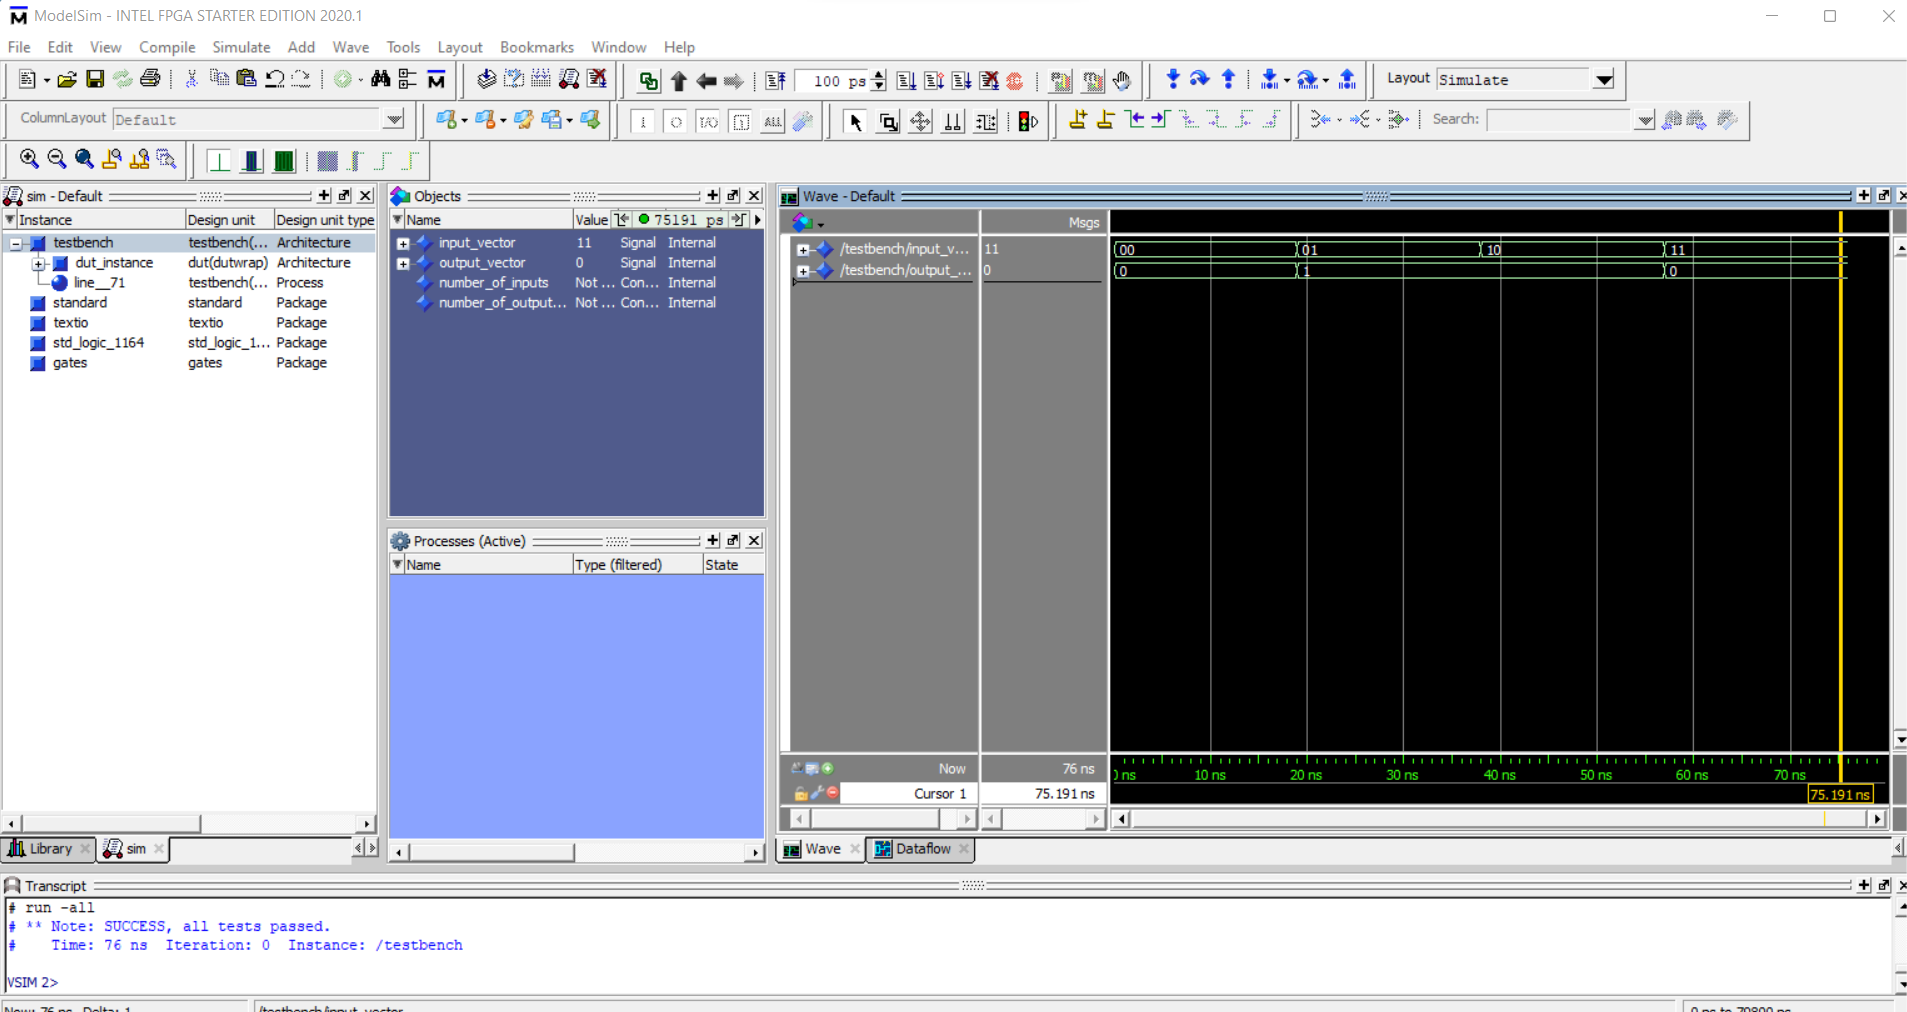
\includegraphics[scale=0.4]{images/XOR_RTL_WAVEFORM.png}  % change scale factor to re-size the image.
  % give a caption.
  \caption{XOR RTL simulation}
  % a label to refer to the figure
  \label{XOR_RTL}
\end{figure}

\begin{figure}[h]
\centering
  % include graphics (can include eps, jpg, pdf ...)
  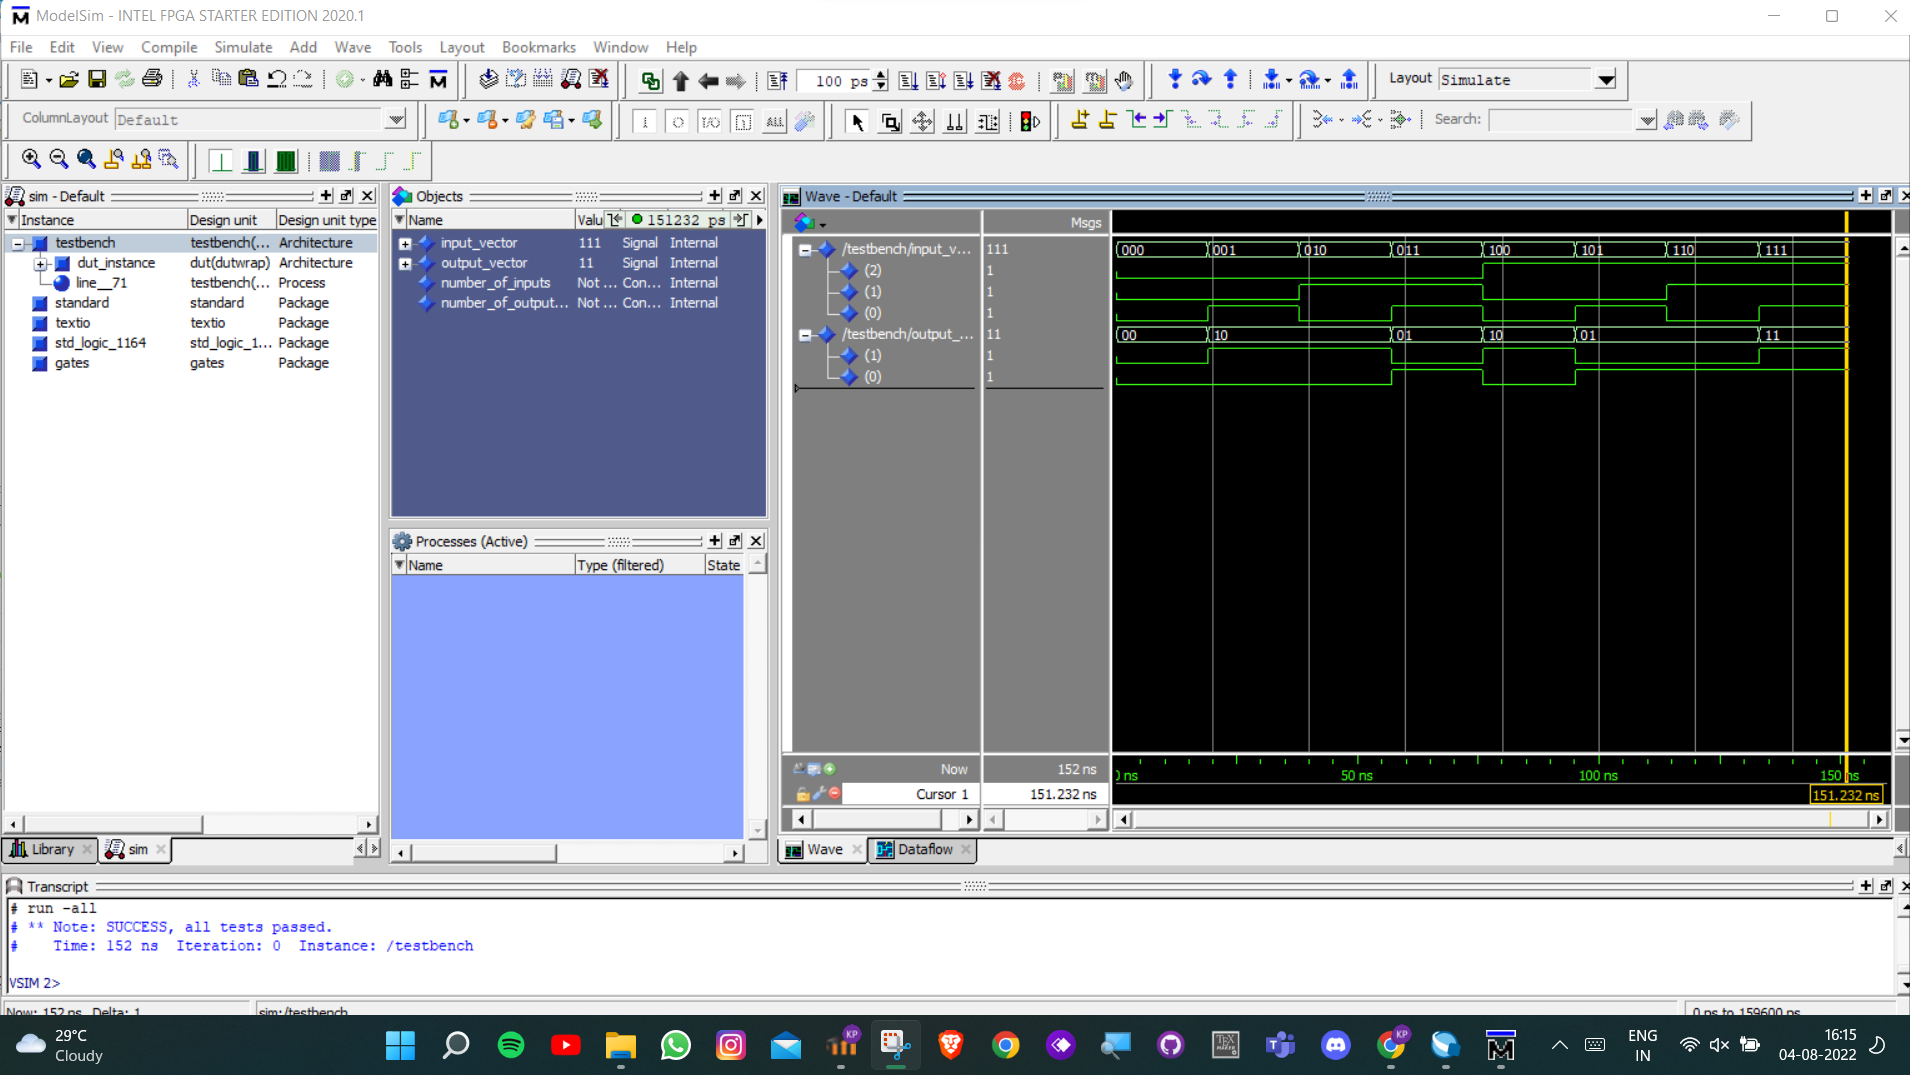
\includegraphics[scale=0.4]{images/FULLADDER_RTL_WAVEFORM.png}  % change scale factor to re-size the image.
  % give a caption.
  \caption{Full Adder RTL simulation}
  % a label to refer to the figure
  \label{Full_adder_RTL}
\end{figure}




\end{document}